% !TEX root = writing_version.tex

\label{chp:simulation}
During the course of the master thesis an event driven molecular dynamics (EDMD) simulation code has been developed. The EDMD approach is chosen because the actual dynamics of the system ais required to search for possible memory effects. This means that simulations only probing the phase space of the system, like Monte Carlo (MC) simulation schemes, are not suited.\\ 
Furthermore the discontinuous potential of the hard spheres is an obstacle not easy to face in regular molecular dynamics (MD) schemes, where the Newtonian equations of motion for the particles are numerically integrated. As the EDMD approach even requires these discontinuitie it is very well suited for the purpose at hand.\\ 
The key points of the program, possible extensions and a thorough testing are presented in the following, starting with the units of the simulation, which are also used throughout this thesis. They are $\sigma$ the sphere diameter as the unit of length, $m$ the mass of a particle as the unit of mass, $k_B T$ as the unit of energy and resulting from these $\delta t = \sqrt{m / (k_B t)} \, \sigma$ as the unit of time.

\section{Algorithm and simulation details}
\label{sec:simulation}
%EDMD and Simulation details
In this section we will highlight the main differences to regular MD simulation schemes, which are an other main tool to probe the dynamics of molecular systems. Furthermore we will stick to the hard sphere example when discussing the EDMD simulation, but it can be kept in mind that the approach allows to simulate all systems governed purely by potentials made of step functions.\\
 
The decisive difference between EDMD simulations and regular MD schemes is that, instead of evaluating all pair and external forces on each particle and then evolving the whole system accordingly to the next time step, EDMD simulations do not use a predefined time step but instead the system is evolved from one event to the next one, where the next event is defined by the next collision of two particles within the simulation box.\\

The employed event prediction algorithm follows closely the approach proposed by Bannerman et al.\cite{Bannerman2014} which is discussed in the next section.

\subsection{Event driven molecular dynamics (EDMD)}
\label{sec:EDMD}
For the prediction of events in EDMD simulations an overlap function $f_{ij}(t)$ between particles i and j is defined, where the squared quantities are used merely because they are easily accessible.\\
\begin{align}
f_{ij}(t) & \coloneqq  | \vec{r}_j(t) - \vec{r}_i(t) |^2 - \sigma^2\\
          & \; \; \, \vrule
  \begin{aligned}[t]
    \quad \text{with} \quad \vec{r}_i(t) &= \vec{r}_i(t_0) + (t-t_0) \; \vec{v}_i(t_0) \, \text{,}\\
    \Delta t \coloneqq & \; t-t_0  \, \text{,} \\ 
    \vec{v}_{ij}(t) &\coloneqq  \vec{v}_j(t) - \vec{v}_i(t) \, \text{,}\\
    \vec{r}_{ij}(t) &\coloneqq  \vec{r}_j(t) - \vec{r}_i(t) \, \text{,}\\
    \Leftrightarrow \quad \vec{r}_{ij}(t) &= \vec{r}_{ij}(t_0) + \Delta t \; \vec{v}_{ij}(t_0)
  \end{aligned}\\
f(t)  & = ( \vec{r}_{ij}(t_0) +  \Delta t \;  \vec{v}_{ij}(t_0))^2 -\sigma^2 \\
\label{eqn:overlap_f}
f(t)  & = |\vec{r}_{ij}(t_0)|^2 + \Delta t ^2 \; |\vec{v}_{ij}(t_0)|^2 - 2 \Delta t \; \vec{r}_{ij}(t_0) \cdot \vec{v}_{ij}(t_0)  -\sigma^2
\end{align}  

The overlap function has the property that it is negative for two particles being closer than their diameter, zero at collision and positive if neither overlapping nor touching. The task to calculate the next collision thus is to calculate the roots of \autoref{eqn:overlap_f}.\\

Solving for $\Delta t$ with $rr \coloneqq |\vec{r}_{ij}(t_0)|^2  $, $vv \coloneqq |\vec{v}_{ij}(t_0)|^2  $ and  $ rv \coloneqq \vec{r}_{ij}(t_0) \cdot \vec{v}_{ij}(t_0) $ has the solution given in \autoref{eqn_delta_t_solution}.
\begin{align}
0 &= rr + vv \; \Delta t ^2  - 2 rv \; \Delta t  -\sigma^2 \nonumber\\
\Leftrightarrow \quad 0 &= \Delta t ^2 - \frac{2rv}{vv} \; \Delta t + \frac{rr - \sigma^2 }{vv} \nonumber\\
\label{eqn_delta_t_solution}
\Leftrightarrow \, \, \Delta t &= - \frac{rv}{vv} \pm \sqrt{\left(\frac{rv}{vv}\right)^2 - \frac{rr - \sigma^2 }{vv}}
\end{align}

But a caveat when executing on a floating point machine is present as can be seen when considering which solution is the relevant one. For a possible collision it is necessary that the two particles move towards each other or mathematically $rv<0$ as the relative velocity is required to be opposite to the relative position.\\

Further the quadratic formula has two solutions, corresponding to the beginning and the ending of the overlap. Because the entry is prior to the exit we further conclude that we are interested in the smaller solution, that is
\begin{align}
\label{eqn:collision_prediction_pre}
\Delta t &= \frac{ - rv - \sqrt{ (rv)^2  - vv (rr - \sigma^2 )} }{vv} \; \text{.}
\end{align}
Now for the case where the distance of the spheres is already close to the diameter of the spheres we find $(rv)^2 \gg (rr-\sigma^2)$, which results in a cancellation of two large numbers leaving a small number. Floating point number operations are inherently badly suited for this as they tend to large inaccuracy in this case. But rewriting \autoref{eqn:collision_prediction_pre} by making use of the third binomial formula leads to the mathematically identical expression
\begin{align}
\label{eqn:collision_prediction}
\Delta t &= \frac{(rr - \sigma^2 )}{ - rv + \sqrt{ (rv)^2  - vv (rr - \sigma^2 )}} \; \text{.}
\end{align}
Comparably \autoref{eqn:collision_prediction} does not contain a cancellation of the type seen before and hence is better suited for the use in the computer simulation as stated by Goldberg 1991\cite{Goldberg1991}.\\

The event prediction algorithm proposed by Bannerman et al.\cite{Bannerman2014} works by differentiating 4 cases:
\begin{enumerate}
\item If $rv>0$ the particles move away from each other leading to a collision time of $\Delta t = \infty$
\item If $rr<\sigma^2$ an overlap is present resulting in an immediate collision time of $\Delta t = 0$
\item If $(rv)^2  - vv (rr - \sigma^2 ) \leq 0 $ the two particles miss each other, including touching without momentum transfer, resulting in a collision time of $\Delta t = \infty$
\item If none of the before is true the particles collide and $\Delta t$ is calculated by \autoref{eqn:collision_prediction}.
\end{enumerate}

All possible collision times for a particle are then stored in a queue that is sorted by the event times and is called particle event list (PEL). From the PEL the first entry is then passed to the global future event list (FEL).This procedure initially takes place for all particles to set up the system and later on only for those particles involved in the execution of an event.\\

While this is the simplest description in \autoref{sec:implemetation} the implementation of some widely used measures to reduce redundant calculations and the use of a cell system to reach $\mathcal{O}(N)$ computation time are further discussed.\\

An important detail to take care of is the possibility of scheduled events which have become invalid due to an earlier collision of one of the particles. This is handled by assigning an interaction count to each particle that is stored at precalculation time with the event. When the event is drawn from the FEL and the interaction count of one of the particles has increased in the meantime, the event is said to be invalidated. Depending on which particle had an event in the meantime the invalidation either causes no action or a recalculation of new events.

\subsection{Details concerning the implementation} 
\label{sec:implemetation}
%Add Details of for example FEL, and backupevent handling, double time precision, reset sim
As the simulation code is based on an earlier Monte Carlo code for hard spheres a complete walk through the whole program would become quite extensive. Hence we will focus on key points to understand the details of the simulation program. Furthermore differences to the MC program are mentioned for the readers that are familiar with it.

\subsubsection{The \textit{Event} struct}
\label{sec:event_struct}
We start with the basic \textit{Event} struct which includes 6 entries that are shown in \autoref{tab:event_entries}.
\begin{table}[h!]
\centering
\begin{tabular}{c|c}
\textbf{Datatype} & \textbf{Name of entry}\\ \hline
(double) & time \\
(int) & event\_type \\
(Particle*)  & particle \\
(void*) & partner \\
(int) & particle\_count \\
(int) & partner\_count \\
\end{tabular}
\caption[\textit{Event} struct content]{Content of the \textit{Event} struct.}
\label{tab:event_entries}
\end{table}
The \textit{time} variable holds the time for when the event is scheduled in the future. The \textit{event\_type} variable is either set to 0 or 1 and indicates if the event is a cell transfer or a collision of two particles, respectively. To include hard walls or other elements further types of events can be defined.\\
The \textit{particle} variable is a pointer to the particle for which the event has been precalculated, while the \textit{partner} variable is defined as a void pointer, allowing it to either be interpreted as a particle pointer for the collision type event or as an integer pointer to the index in the current cells' neighbors list for transfer events.\\
In the last two rows the interaction counts for particle and partner are listed as well. As the destination cell in a transfer event does not require an interaction count the \textit{partner\_count} variable is only used for collision events.\\

The \textit{event} struct is used for all events throughout the simulation. For read and write operations with the HDF5 file format, the struct \textit{event\_data} is available which uses only indexes instead of pointers.

\subsubsection{The \textit{Particle} class}
\label{sec:particle_class}
The \textit{Particle} class is comparable to the one from the MC code basis. Its MC related attributes have been removed and additional key variables and concepts will be discussed in the following.\\

First a vector storing events called \textit{backupEvents} has been added to make it possible to store events from the precalculation for the case of the first event being invalidated. The idea of reusing events is discussed in many publications, for example that the memory cost increases linearly with more backup events while the speedup does not increase much for more than two stored events Bannerman et al. 2011\cite{Bannerman2011}. It also has been argued that the added complexity can not account for the increase in efficiency Donev et al. 2005\cite{DONEV2005}.\\ 
However in our own simulations a calculation time reduction of more than 10\% was observed and the cost of complexity and memory was seen as moderate. The difference might be explained by the fact that the systems under consideration in this thesis have a rather large particle density, leading to more invalid collisions.\\

In the context of reusing precalculated results, it should also be mentioned that after a cell transfer the recalculation of events can be reduced to possible partner particles of only the new neighboring cells, leading to only 1/3 of the calculation time in this case. But as mentioned systems under consideration are very dense resulting in little transfer events often only constituting less than 5\% of all executed events. Thus the increase in efficiency was assumed to be to costly on the complexity side, and not implemented. But for sparse systems it might make sense to include an \textit{updatePEL()} routine as transfers are more frequent.\\

Also key differences to the former MC particle type are the variables \textit{total\_interactions} and \textit{particle\_delayed\_time}. The first is the variable for book keeping of interactions, while the second represents the event driven character of the simulation. Because each particle only moves on purely ballistic trajectories until an event occurs it is not necessary to keep all particle positions and velocities synchronized in time. Quite on the contrary it would mean executing extra operations with extra calculation time and extra rounding errors.\\
To take the whole configuration to one point of time, the \textit{transferToTime()} function of the particle is provided. This is obviously necessary for measurements including snapshots.\\

As mentioned before the system behaves chaotic even under slightest changes like a rounding error from an extra floating point operation. A result of this is that measuring at different rates during a simulation changes the simulation trajectory quite a bit. It is observed in \autoref{sec:precision} that the system may keep close to the undisturbed trajectory for about 50-100 events/particle. As it is of desire to measure quantities and take snapshots without disturbing the simulation, the program employs copies of the configuration being costly in terms of memory but making simulation resets or higher sampling rates at interesting points possible within a well defined trajectory.\\ 

The measurement without perturbing the system is implemented by making a backup copy of the working configuration just before a measurement is taken. The working trajectory then is disturbed by the measurement and afterwards replaced with its state before the measurement from the backup configuration.\\
A second copy is carried throughout the simulation including the full simulation state, while the first only includes the particle configuration. To save a state during the simulation and reset to just the same point at any later time might be useful for example to do a committer analysis, where a cluster at different stages is sampled multiple times with different perturbations.

\subsubsection{The \textit{Box} class}
\label{sec:box_class}
The box of the simulation remained in principle the same as in the previous MC code. A new element is the \textit{neighbors\_lookup} table, which contains the indices to the elements in the cells' array \textit{neighbors}, where pointers to the cells that share a surface are stored. It is used to identify which cell a particle has to be transferred to during a cell transfer event.\\

Furthermore the \textit{Update()} routine now takes care of all quantities depending on the length of the box, and the \textit{rescale()} routine is a simple rescaling of the edge lengths with an additional \textit{Update()} call.

\subsubsection{The \textit{Scheduler} class}
\label{sec:scheduler_class}
While the aforementioned elements of the program are also required for the EDMD simulation, the \textit{Scheduler} class certainly contains the most distinct parts of the program. It keeps track of all events to come, predicts new events and orchestrates the execution of the events. The essential functions are discussed in the following subsections while some basic properties are shortly highlighted here.\\

First of all the \textit{Scheduler} holds the future event list (FEL) in which at least one event per particle is stored. As discussed within \autoref{sec:particle_class} the simulation is capable of saving the complete state of a trajectory, including all precalculated events. For this purpose the \textit{reset\_FEL\_array} is available. Furthermore the \textit{Scheduler} includes the \textit{global\_time} variable that holds the latest event execution time.\\

We may also note the importance to preallocate all arrays that are used in the event calculations for the efficiency, because the collision prediction routine is executed about 30 times per step and particle, easily accounting to a few billion function calls during a small simulation.

\subsubsection{\quad \textit{Scheduler::predictTransfer()}}
As the name suggests this function predicts the next cell transfer of a particle due to its movement. For this it calculates the position of the particle at global time, which for a valid state of the simulation always lies within it's cell. Denoting for each dimension $i$, the position of a particle within its cell by $r_i$, it's velocity by $v_i$, and the cell's length by $l_i$, we can write for each dimension the equations
\begin{align}
t_{i1}=-\frac{r_i}{v_i} \quad \text{and} \quad t_{i2}=\frac{l_i-r_i}{v_i} \; \text{,}
\end{align}
which describe the times $t_{i \, 1/2}$ when the particle pierces the cell's left and right boundaries in dimension $i$. A negative time corresponds in this case to a boundary crossing in the past, a time comparable to 0 means that the particle is on the edge of its cell and a positive time means that the boundary crossing lies in the future. By going through the different possible cases for $t_1$ and $t_2$ we find the resulting next crossing time for each case as shown in \autoref{tab:crossing_times}.
\begin{table}[h]
\centering
\begin{tabular}{c|c||c|c}
$t_1$ & $t_2$ & Result & Case \\ \hline
> & > & invalid & - \\ \hline
> & = & $t_{\text{crossing}} = t_1$ & 0 \\ \hline
> & < & $t_{\text{crossing}} = t_1$ & 1 \\ \hline
= & > & $t_{\text{crossing}} = t_2$ & 2\\ \hline
= & = & invalid & - \\ \hline
= & < & $t_{\text{crossing}} = t_1$ & 3 \\ \hline
< & > & $t_{\text{crossing}} = t_2$ & 4 \\ \hline
< & = & $t_{\text{crossing}} = t_2$ & 5\\ \hline
< & < & invalid & - \\ \hline
\end{tabular}
\caption[Cell boundary crossing conditions]{Possible results for left and right crossing time with resulting choice of next crossing time. >, = and < are to be read as for example $t_1 > 0$. The case indicates the case number within the simulation code.}
\label{tab:crossing_times}
\end{table}

By collecting the next crossing times for each dimension and taking the minimum of these times the exit time of the particle from its cell is determined.\\

The return value of the routine is an \textit{Event} where the partner is a pointer to the corresponding entry in the box' \textit{neighbors\_lookup} table. The index lies between zero and five for to the six possible neighbor cells sharing a surface with the current cell of the particle. Each valid case represents a distinct neighbor cell and its index within the cell's \textit{neighbors} array is clearly defined by the cell setup routines. The indices within the neighbors array are matched with the defined cases is \autoref{tab:cell_neighbor_index}. 

\begin{table}[h]
\centering
\begin{tabular}{c|c|c|c}
dimension & boundary & case & index \\ \hline
x & front & 0 & 12 \\
 & back & 1 & 13 \\ \hline
y & front & 2 & 10 \\
 & back & 3 & 15 \\ \hline
z & front & 4 & 4 \\
 & back & 5 & 21 \\
\end{tabular}
\caption[Lookup table of cell neighbor indices]{Overview of the cells' \textit{neighbors} indices directly sharing a surface for 3 dimensions. As the indices hardly follow any simple pattern they are explicitly noted at this point. Obviously the cell consists of a front and a back boundary in each dimension. The corresponding case numbers are identical to the ones from \autoref{tab:crossing_times}.}
\label{tab:cell_neighbor_index}
\end{table}
\FloatBarrier

\subsubsection{\quad \textit{Scheduler::predictCollision()}}
The prediction of collision times has already been discussed in \autoref{sec:EDMD}. The implementation in the program first calculates all necessary scalar products while accounting for the periodic boundary conditions, and in a second step returns the collision time depending on the case at hand.\\

While the here presented algorithm is only valid for single sized particles it can be extended to polydisperse systems as is shown in \autoref{sec:extension_radius}.\\

As this routine is executed throughout the simulation very often it has been tried to optimize its efficiency as far as possible. For example calculating only necessary results for the next case differentiation has been tried but without significant increase in efficiency and for better readability the prior version has been used instead. In either case if more efficient calculations are found it is useful to implement them at this point.\\   

\subsubsection{\quad \textit{Scheduler::setupFEL()}}
This routine fills the FEL of the simulation. For this purpose it iterates through all particles and calls \textit{setupPEL()} for each of them. The PEL in turn is set up by predicting the next cell transfer as well as the next collisions with all particles within the $3^d$ cells in $d$ dimensions directly surrounding the particle. From all predicted events only such with finite times are then written to the \textit{backupEvents} vector that is the PEL of the particle.\\
For the FEL only the top event of each particle's PEL is then used. Because other events from the PEL might move on to the FEL at later times the top event that was pushed to the FEL has to be erased from the PEL.\\

\subsubsection{\quad \textit{Scheduler::executeTransfer()}}
The execution of a transfer event is accomplished by the particles \textit{MoveBetweenCells()} routine. The departure cell is taken as the event particles own cell, while the information about the destination cell is contained in the event's \textit{partner} variable. It points to an address within the look up table of the box where the index of the destination cell in the departure cell's neighbor array is deposited.\\

\subsubsection{\quad \textit{Scheduler::executeCollision()}}
The outcome of a collision between particle 1 and 2 with corresponding position and velocity can be derived by momentum and energy conservation too be 
\begin{align}
\label{eqn:collision_result}
\vec{v}_1^{\,'} = \vec{v}_1 + \left( \frac{\vec{r} \cdot \vec{v} }{\vec{r} \cdot \vec{r}} \right) \vec{r}_{12}
\end{align}
While \autoref{eqn:collision_result} is not directly depending on the radius, an indirect dependence  by the collision time and configuration at which \autoref{eqn:collision_result} is evaluated persists. The generalization to arbitrary masses is also given in \autoref{sec:extension_radius}.
 
\subsubsection{\quad \textit{Scheduler::executeEvent()}}
The execution of an event works in multiple steps. At first the topmost \textit{Event} is copied from the FEL where it is deleted. Next the validity of the interaction counts of both particle (\textit{cond1}) and its partner (\textit{cond2}) are evaluated. The validation is nothing else than a comparison of the interaction counts when the event was scheduled with the present interaction counts. As the conditions are used in the following flow statements they are stored in boolean variables. Furthermore in the case of a transfer event the validation of the partner is not necessary but for better readability performed either way.\\
It follows a distinction between 5 cases which are given by:
\begin{description}
\item[Valid transfer (\textit{event\_type}==0 and \textit{cond1}) ] \hfill \\ The transfer is executed, the global time is evolved to the event time, the particle's PEL is rebuilt and it's next event pushed to the FEL.
\item[Valid collision (\textit{event\_type}==1 and \textit{cond1} and \textit{cond2}) ]\hfill \\ The collision is executed, the global time is evolved to the event time, for both participating particles new PEL's are built and each top event is pushed to the FEL.
\item[Invalid transfer (\textit{event\_type}==0 and not \textit{cond1})] \hfill \\ The particle must have had an interaction previously where a new event for it was scheduled, thus no action is taken.
\item[Invalid collision due to particle (\textit{event\_type}==1 and not \textit{cond1})] \hfill \\  The particle must have had an interaction previously where a new event for it was scheduled, thus no action is taken.
\item[Invalid collision due to partner (\textit{event\_type}==1 and not \textit{cond2})] \hfill \\  Only the partner had an interaction previously where a new event for it was scheduled, thus a new event for the particle is required. As the particle had no further interactions, the \textit{backupEvents} are still valid and its first entry is pushed into the FEL. In case no backupEvents are stored the PEL is rebuilt and its first entry pushed to the FEL instead.
\end{description}
The order of the cases might be exchanged, except for the last two. This is because the last one indirectly assumes \textit{cond1} to be true, which is guaranteed only by the case before.\\

Furthermore the routine counts the number of each case, to monitor numbers of collisions, transfers and invalidated cases by type. This is not required by the simulation but can be helpful for understanding the system and simulation.\\

\subsection{Simulation periphery}
\todo{Well either make it a little nicer or maybe leave it out}
For the simulation to work also some more surrounding is required. The corresponding parts of the simulation are only briefly discussed.
 
\subsubsection{Inout and ch5md}
As suggested by the names, the first comprises the read and write routines of the simulation, while the later one holds routines dealing with the h5md format. The used data types are mostly single figures, arrays, variable length arrays and tables.

\subsubsection{Setup}
The setup routines are called mainly at the beginning of a simulation to either set up a simulation from a file or to completely start a new simulation.

\subsubsection{Tools}
This is the toolbox of the simulation holding routines to measure quantities like mean squared displacement, radial distribution functions and also the cluster finding routine. It also contains an overlap and minimal distance function used within the simulation during compression.

\section{Testing of the simulation code}
\label{sec:probe}
To probe the simulation dynamics we measured the long time diffusion constant and the radial distribution function of the stable hard sphere liquid, as there are many measurements available in the literature to compare with.

\subsection{Diffusive behavior}
\label{sec:diffusion_probe}
The diffusive behavior of particles in a liquid usually can be separated in three distinct parts. First the short time diffusion which can be understood as the random movement of the particles within their momentary cage within the fluid. Second a sub diffusive phase in which the particles are repelled for the first time by their nearest neighbors. And third the long time diffusion to describe the random propagation of the particle through the fluid over time.\\
   
As the ballistic hard sphere system enters into the long time diffusion almost at once only this is really measurable. By assuming a diffusive process we have the expectation that the average mean squared displacement (MSD) of a particle can be well described by 
\begin{align}
\label{eqn:diffusion}
\langle x^2 \rangle(t) = 2 \, d \, D \, t  \, \text{,}
\end{align}
where $\langle x^2 \rangle$ is the expectation value of the MSD, $d$ the number of spatial dimensions, $D$ the characteristic diffusion constant, and $t$ the time by which the system has evolved.\\

By measuring $\langle x^2 \rangle (t)$ and making a linear regression to the data points we can find the Diffusion constant $D$.

To probe the simulation code, systems as characterized in \autoref{tab:system_diffusion} have been used. The equilibration phase has been carried out already at the final volume fraction up to $\eta_f = 50\%$, while above this an initial volume fraction of $\eta_i = 45\%$ has been used to obtain a fluid rather than a solid during the equilibration phase. As some measurementes are within the metastable regime, it has been checked that no clusters were present in the box during the measurement as they would reduce the averaged diffusion.\\

The resulting diffusion constants depending on the fluid volume fraction are shown in \autoref{fig:diffusion_const} alongside values obtained from the literature, for a similar system.\\

\begin{figure}[h]
\centering
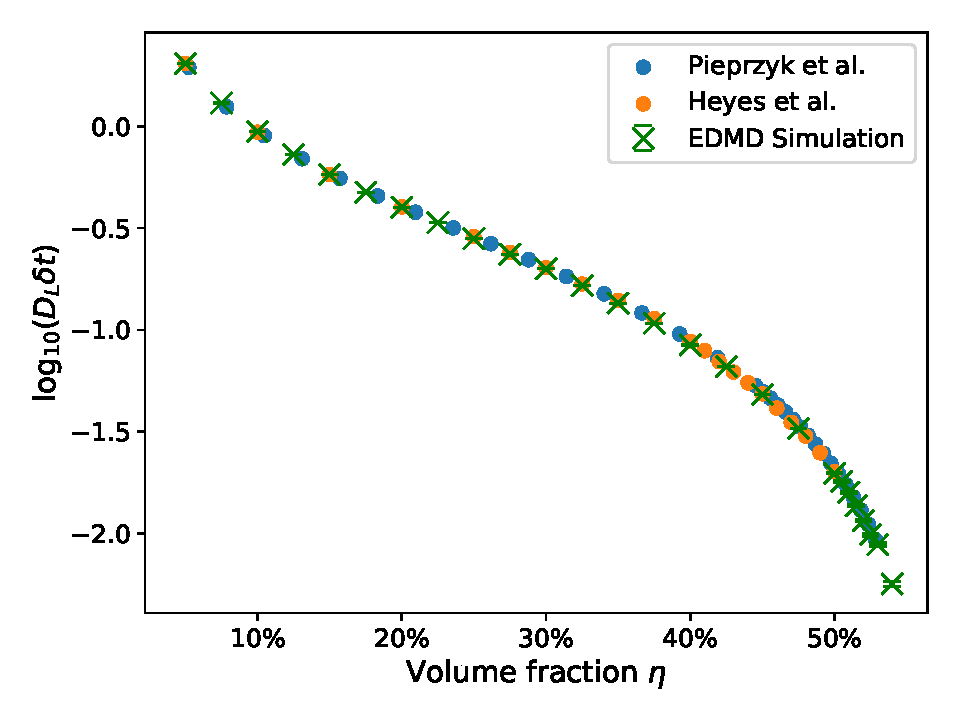
\includegraphics[width=0.7 \linewidth]{diffusion_probe.pdf}
\caption[Long time diffusion constant at varying volume fractions]{Logarithmic plot of long time diffusion constant of the hard sphere liquid as measured in our own simulations as well as measurements from the literature\cite{Pieprzyk2019},\cite{Heyes2007}.}
\label{fig:diffusion_const}
\end{figure}

As it can be seen the EDMD simulation is very well capable of reproducing the diffusion constant for the hard sphere liquid, and therefore we expect the dynamics of it to accurately represent the purely ballistic hard sphere system.\\


\begin{table}[h]
\centering
\begin{tabular}{c|c}
Parameter & Value \\ \hline
N & 16384 \\
eq\_steps/particle & 5000 \\
pr\_steps/particle & 20000 \\
$\eta_i$ & 5\% ... 50 \% \\
$\eta_f$ & 5\% ... 54 \% \\
\end{tabular}
\caption[Simulation parameters for diffusion measurement]{Input parameters of diffusion test systems.}
\label{tab:system_diffusion}
\end{table}





\subsection{Radial distribution function}
\label{sec:RDF_prob}
A further well known quantity for the hard sphere system is the radial distribution function. As a theoretical prediction the Percus-Yevick approximation can be used to compare with, also it would be possible to compare with Monte Carlo simulations of the hard sphere system. In \autoref{fig:rdf_overview} an overview for a range of volume fractions is shown from the same simulations used in \autoref{sec:diffusion_probe}. Clearly visible is that no particles enter within the diameter of the spheres. Further for higher volume fractions the liquid shells become very well visible. At very high volume fraction we also find that  new peak arises below $r = 2 \sigma$.
\begin{figure}[h]
\centering
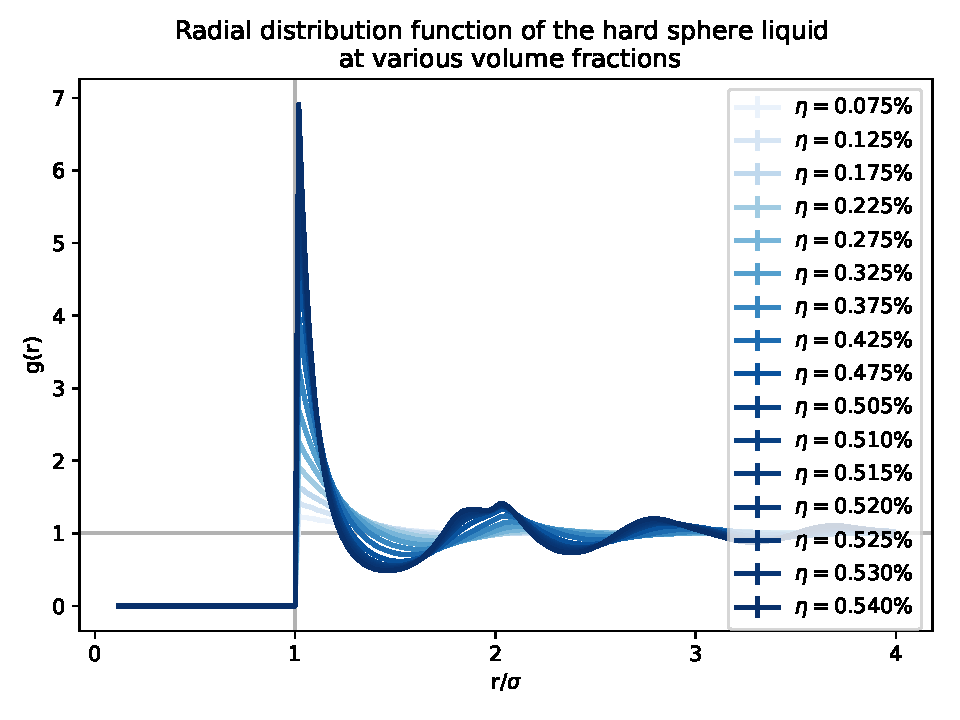
\includegraphics[width=0.7 \linewidth]{RDF.pdf}
\caption[Radial distribution functions at varying volume fractions]{Radial distribution functions for a range of volume fractions. The coloring corresponds to the used volume fraction.}
\label{fig:rdf_overview}
\end{figure}

To compare with Percus-Yevick approximation the radial distribution function for two single volume fractions is shown with the corresponding theoretical solution in \autoref{fig:rdf_py}.
\begin{figure}[h]
\centering
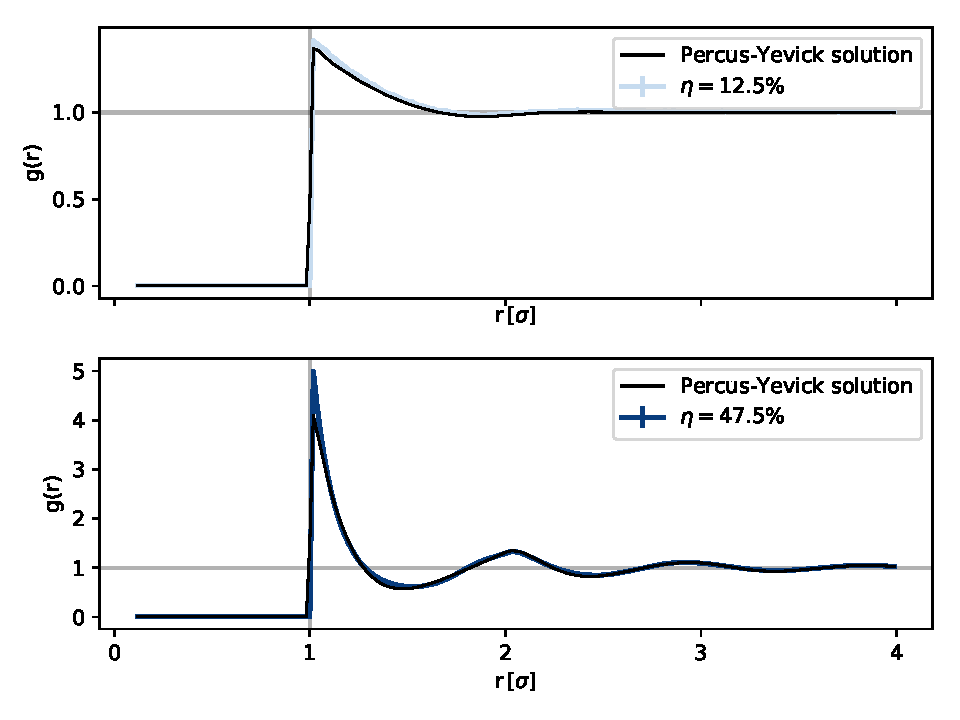
\includegraphics[width=0.7 \linewidth]{RDF_percus_yevick.pdf}
\caption[Radial distribution function with Percus-Yevick solution]{Radial distribution function for the hard sphere system at a low and at a high volume fraction of the liquid together with the theoretical prediction from the Percus-Yevick approximation.}
\label{fig:rdf_py}
\end{figure}

As highlighted for example in \cite{Hansen2006} the theoretical approximation has some flaws as can be seen with $g(r)|_{r=1\sigma}$ being too low for the Percus-Yevick approximation. But overall the two radial distribution functions follow each other rather closely giving confidence that the developed simulation code is capable of producing accurate data in other contexts as well.\\

\section{Estimate of required resources}
\label{sec:resources}
To choose system parameters reasonable, calculation times and file sizes of the simulation have been characterized. This was of interest as the program was supposed to run on the NEMO high performance computing cluster which puts hard boundaries on calculation times which when trespassed can cause tremendous loss of data if not correctly caught by the program.\\
 
\subsection{Calculation time estimate}
\label{sec:calc_times}
The calculation time of the program was tested for a large range of different system sizes up to almost 9 million particles in the fluid state. As can be seen in \autoref{fig:calc_time} the calculation time increases proportional to the system size for the execution of a step as well as for a measurement of the fluid system. The calculation cost being of $\mathcal{O}(N)$ enables the study of large systems. Furthermore from the slope an expectation for the execution time of a single event can be deduced, as well as an expectation for the time necessary for a measurement. As discussed on the example of \autoref{fig:calc_q6q6} the dependence of the measurement routines on the largest cluster size were not seen here, as possible clusters remained rather small during these simulation times.\\

\begin{figure}[h!]
\centering
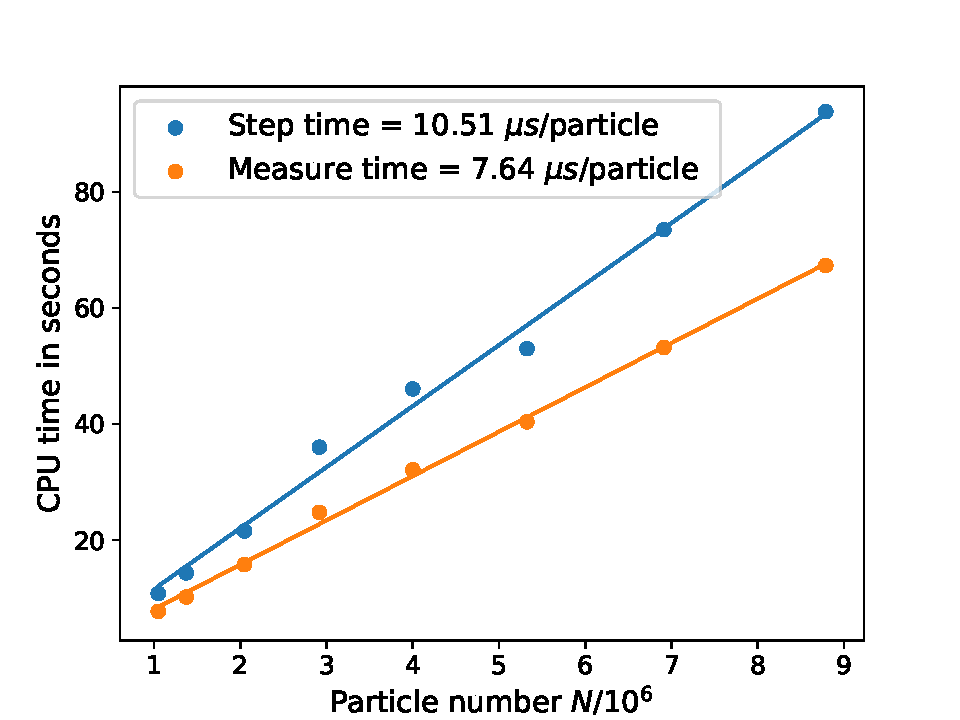
\includegraphics[width=0.7 \linewidth]{Calculation_times_measurement.pdf}
\caption[Calculation time estimate]{Overview of CPU time required for calculating a simulation step, consisting of an event for each particle, and a measurement of relevant quantities for the system. As assumed for a simulation algorithm with $\mathcal{O}(N)$ calculation effort, the data points can be described by a line rather well. As the CPU time is clearly related to the further workload of the CPU during the calculation it is also expected to find fluctuations if the other workload of the machine is not strictly controlled.}
\label{fig:calc_time}
\end{figure}

The effect of larger clusters was only investigated after problems with the runtime of the programs were traced back to these. The q6q6-order parameter routine was tested for larger clusters in a nucleating simulation with about 1 million particles within the box. As can be seen in \autoref{fig:calc_q6q6} the calculation cost of the cluster finding routine can be described with a quadratic dependence on the largest cluster. For an impression what this means we can use the calculation costs of a simulation step from \autoref{fig:calc_time} being about $t_{step} \approx \SI{10}{\mu s \per \text{particle} }$. Therefore the execution of one step takes about $\SI{10}{s}$ for 1 million particles. If a measurement is performed every 10th step, the calculation cost of the measurements without a large cluster remain below 10\%. But as the largest cluster grows to a few hundred thousand particles in size, the measurements can make up 30 \% and more of the calculation cost, or for a fixed number of steps, increase the calculation time by about 50 \%. This previously unseen effect lead to actual data loss as the combination of NEMO's policy and EDMD simulation program did not result in a save shutdown of the program after breaching the wall time limit of four days.\\

\begin{figure}[h!]
\centering
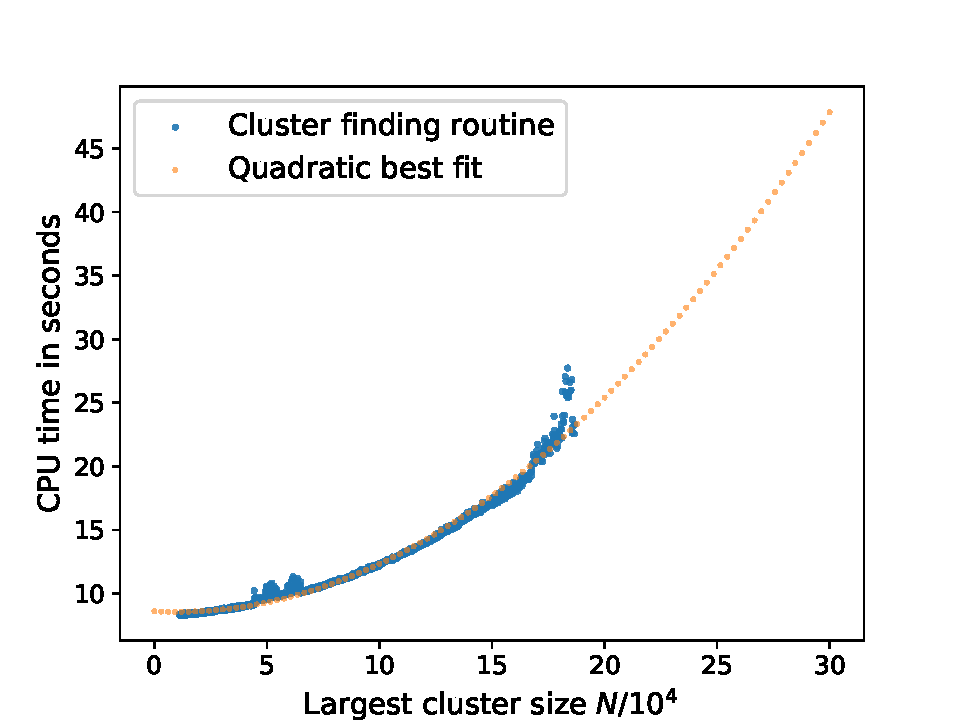
\includegraphics[width=0.7 \linewidth]{q6q6_calculation_time.pdf}
\caption[Quadratic calculation time of q6q6-order parameter cluster finding routine]{Calculation time of the q6q6 order parameter at an increasing largest cluster size during one nucleation, together with the quadratic best fit indicating that the q6q6 routine calculation effort can be approximated by $\mathcal{O}({N_{\text{lc}}}^2)$ where $N_{\text{lc}}$ is the size of the largest cluster.}
\label{fig:calc_q6q6}
\end{figure}


\subsection{File sizes estimate}
\label{sec:file_size}
A further important constraint for the simulations are the produced amount of data. To get an impression of the file sizes, the required memory for snapshots, reset steps and other measurements were measured prior to the actual simulations. The results for a single snapshot containing all positions and velocities of all particles as well as the size of a single simulation reset step containing all positions, velocities, the FEL, all PEL's and all delayed times is shown in \autoref{fig:file_size}. It can be seen that the file size is directly proportional to the system size which clearly expected as each particle adds a further set of positions, velocities etc. to the saved data.\\
The memory costs of other measurements have been left out of \autoref{fig:file_size} as these only amount to substantial file sizes if measurements at about each step for long simulations are done.\\  

\begin{figure}[h!]
\centering
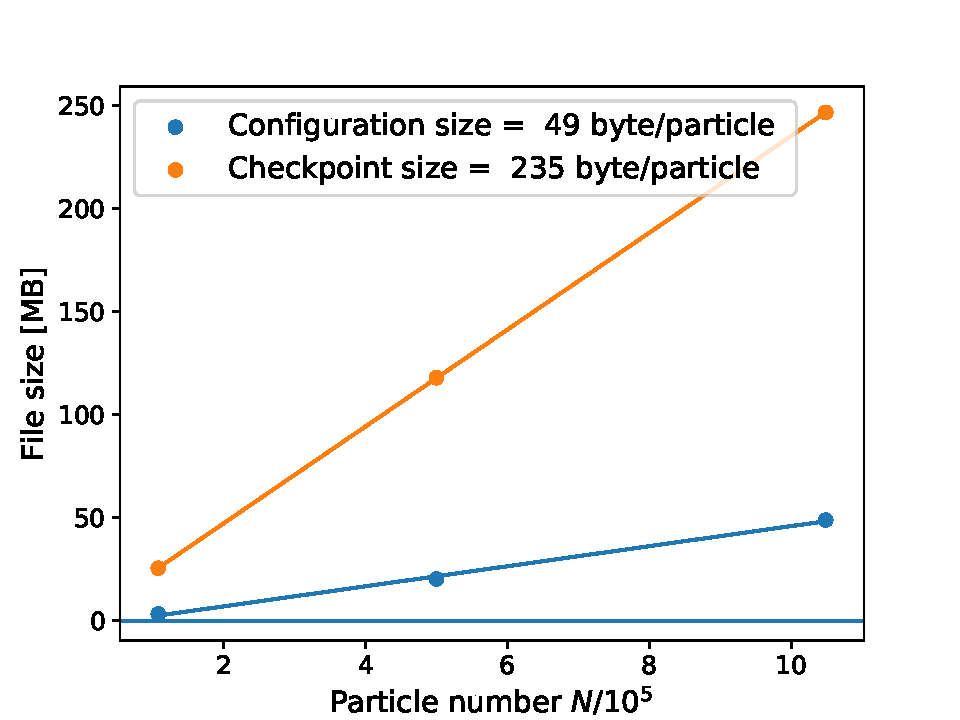
\includegraphics[width=0.7 \linewidth]{File_size.pdf}
\caption[File size estimate]{Overview of file sizes when a single setup on the one hand and a single full simulation on the other hand is saved for comparison reasons together with their corresponding linear regression. While the linear regression for 3 points is statistically not exceedingly meaningful it still remains a useful tool to extract the slope which corresponds to the required memory per particle and snapshot or reset simulation.}
\label{fig:file_size}
\end{figure}

\section{Preliminary data for equilibration test}
\label{sec:data}
The motivation for the simulation code is based on the interest in nucleation rates of the hard sphere system at varying volume fractions. To observe a nucleation the volume fraction of hard spheres has to be changed rapidly from lower ones where the system is in the stable fluid phase to higher ones where a metastable fluid-solid phase exists. If this metastable phase is evolved in time nucleations can be observed as stochastic distributed events. To measure those without effects originating from the handling of the simulation, some parameters were tested within reasonable ranges prior to the data production.\\
For this simulation the equilibration steps as well as the initial density before the volume quench seemed like they could introduce unwanted artifacts, and thus we performed some smaller data series to evaluate if and when these effects might come into play.\\

The used test system is characterized by the figures in \autoref{tab:system_start_parameter_test}.

\begin{table}
\centering
\begin{tabular}{c|c}
Parameter & Value \\ \hline
N & 16384 \\
eq\_steps/particle & 100 ... 20000 \\
$\eta_i$ & 5\% ... 49 \% \\
$\eta_f$ & 54 \% \\
\end{tabular}
\caption[Simulation parameters for testing equilibration step number and initial density]{Input parameters of test systems probing the dependence on equilibration steps and initial density.}
\label{tab:system_start_parameter_test}
\end{table}

The general behavior of the systems is analysed by inspecting the cluster distribution over time. The mean cluster distribution is shown in \autoref{fig:pnt_mean} together with the same data smoothed by a Gaussian filter matrix. The smoothing is used because in a next step the difference between the mean cluster distribution and the cluster distributions with varying simulation parameters is compared, and without smoothing at low count rates only fluctuations are visible.\\


\begin{figure}[h!]
\centering
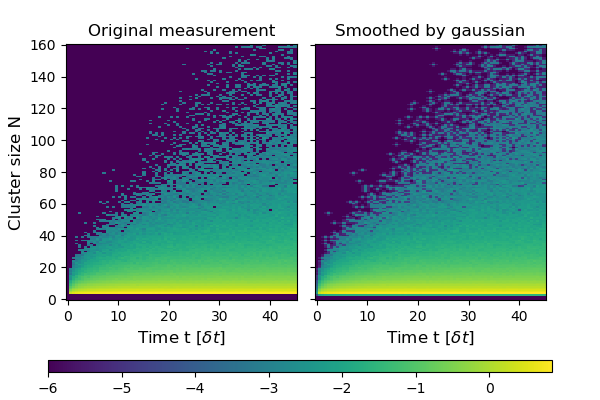
\includegraphics[width=0.7 \linewidth]{mean_pnt.png}
\caption[Gaussian filter applied to cluster size distribution]{Heat map of the mean cluster distribution over time. The diagram encompasses 800 trajectories of 16384 particles each. The coloring indicates the logarithm of the mean cluster occurrence corresponding to a probability in the stationary case.}
\label{fig:pnt_mean}
\end{figure}

From \autoref{fig:pnt_mean} we can see how the system behaves after a volume quench into the metastable region. In the liquid rarely any clusters are present and thus directly after the quench no clusters are present either as the spatial configuration requires time to rearrange into clusters. In the later evolution we see how clusters form, and soon after begin to nucleate leaving the range of the diagram.\\

To compare simulations with varying parameters the quantity defined in \autoref{eqn:pnt_delta} is used, where complications with zero values are circumvented by fixing these values below the regular signal.\\ Three samples of this comparison are shown in \autoref{fig:pnt_eq_step_comparison} and \autoref{fig:pnt_eq_step_comparison}. The coloring indicates $\Delta_{p(N,t)}$ defined in \autoref{eqn:pnt_delta}. As mentioned above the quantities $p_i(N,t)$ and $\langle p(N,t) \rangle$ have been smoothed by a Gaussian filter, because the number of samples included, with 100 trajectories per series, were not sufficient to produce smooth distributions at the given sampling rate. Thus without smoothing only fluctuations would be visible.\\ 

\begin{align}
\label{eqn:pnt_delta}
\Delta_{p(N,t)} = \text{log} \left( \left| \frac{p_i(N,t)}{\langle p(N,t) \rangle} -1 \right| \right)
\end{align}

\begin{figure}[h!]
\centering
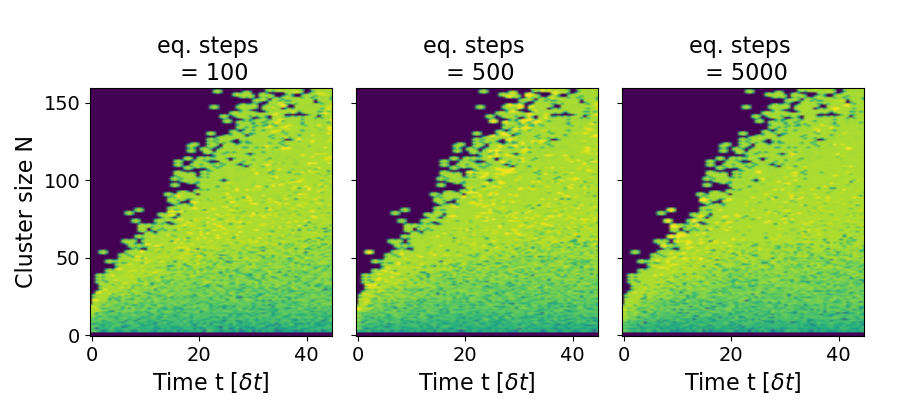
\includegraphics[width=0.7 \linewidth]{pnt_comparison_eq_steps.png}
\caption[Heat maps of differences under variation of equilibration step number]{Heat map of differences between the cluster distributions within simulations carried out with varying the length of the equilibration phase. The quantity used for coloring is defined in \autoref{eqn:pnt_delta}, where yellow indicates a large difference while blue indicates a small difference. Providing a legend of the coloring is omitted as $\Delta_{p(N,t)}$ has no further use than to indicate differences and actual values do not add any use.}
\label{fig:pnt_eq_step_comparison}
\end{figure}


\begin{figure}[h!]
\centering
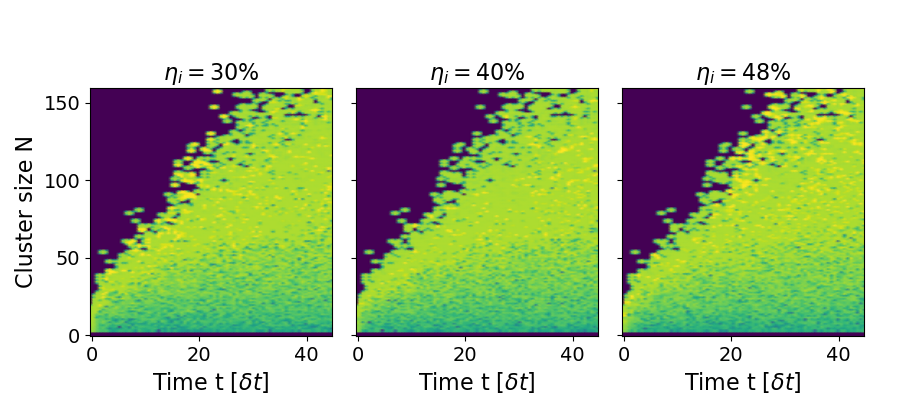
\includegraphics[width=0.7 \linewidth]{pnt_comparison_rho.png}
\caption[Heat maps of differences under variation of initial density]{Heat map of differences between the cluster distributions within simulations carried out with varying the volume fraction of the liquid during the equilibration phase. The quantity used for coloring is defined in \autoref{eqn:pnt_delta}, where yellow indicates a large difference while blue indicates a small difference. Providing a legend of the coloring is omitted as $\Delta_{p(N,t)}$ has no further use as to indicate differences and actual values do not add any use.}
\label{fig:pnt_rho_comparison}
\end{figure}

On first sight none of them differ in their general behavior. Because at t=0 after the quench no clusters have formed yet and also no clusters were present in the stable liquid, the difference between all simulations is zero, indicated by the blue region in the top left corner. The features visible on the edge between the zero region and the nonzero region on the other side are the same, because they are features of the mean distribution carried through. Actual differences not due to fluctuations can only be seen within the green and yellow non-zero region, but none such differences is observed.\\

While it seems like the initial volume fraction of $\eta=0.4$ and $eq\_steps = 5000$ include less irregular fluctuations, dramatic effects from choosing the simulation parameters can be excluded. Interesting in this context are especially the simulations with $eq\_steps = 100$ because after executing 100 events/particle on average, the initial perfect crystal configuration is only on the edge of not being detected anymore. For this reason one could expect that a significant part of these configurations might directly crystallize again, but instead we do not detect any significant difference.\\

A more detailed analysis of the differences is given by calculating the mean nucleation rates assuming classical nucleation theory. This is done for the data shown in \autoref{fig:comparison_nucleation_rates}. The calculations of the rates have been carried out as described in \autoref{sec:induction_times}.

\begin{figure}[h!]
\centering
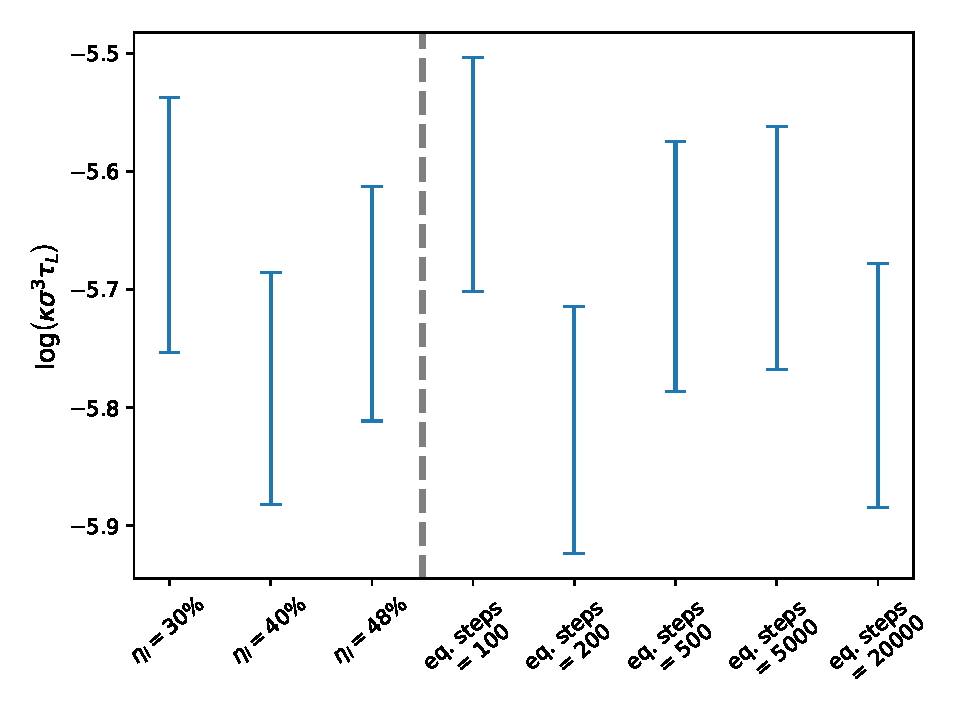
\includegraphics[width=0.7 \linewidth]{nucleation_rate_pre_comparison.pdf}
\caption[Nucleation rates of equilibration test measurements]{Comparison of nucleation rates under CNT assumptions for different initial densities during equilibration with eq\_steps fixed at 5000, as well as varying eq\_steps with $\eta_i$ fixed at 0.45. }
\label{fig:comparison_nucleation_rates}
\end{figure}

As we see, no significant difference in the nucleation rates can be observed even for the extreme short equilibration phase of 100 events per particle. For this bold setting the rate is a little higher, but still in accordance with the other measurements within its statistical uncertainty.\\

Overall we conclude in this chapter that as long as parameters are set within reasonable boundaries, we expect not to have systematic influences of simulation parameters. 

\section{Extensions for future studies}
\label{sec:simulation_ext}
The program at this state is capable of simulating large systems including compression and relaxation. While it has been used to study the nucleation of the monodisperse hard sphere fluid in this thesis, further features have been developed to suit the code for further studies. Polydispersity in the sense of radii and masses have been implemented and roughly tested, as well as individual cluster tracking, to enable detailed study of spatial information about the clusters. These two features are described and their use summarized in the following section.

\subsection{Polydispersity for varying radius and mass}
\label{sec:extension_radius}
Polydispersity has been included in the simulation to make comparison with the real world simpler, as in actual experiments monodisperse spheres are practically not archived. For the implementation the prediction of collisions has to be adjusted. When looking at the derivation of \autoref{eqn:collision_prediction} it is found that $\sigma$ being the former diameter of a sphere in the monodisperse case has to be changed to $\sigma=R_i+R_j$. In the equations the same definitions of scalar products are used as before in \autoref{sec:EDMD}.

\begin{align}
\label{eqn:collision_prediction2}
\Delta t &= \frac{(rr - \sigma^2 )}{ - rv + \sqrt{ (rv)^2  - vv (rr - \sigma^2 )}}
\end{align} 

For a physical model in which the particles are made of some matter with constant density the change of the radius is also accompanied by a change of the mass. This has to be taken into account when assigning the velocities after a collision as written in \autoref{eqn:var_mass}.

\begin{align}
\label{eqn:var_mass}
\vec{v}_i{\,'} = \vec{v}_i + \frac{2 m_j \; (rv)}{(m_i + m_j) \sigma^2} \cdot (\vec{r}_j - \vec{r}_i) \nonumber \\
\vec{v}_j{\,'} = \vec{v}_j + \frac{2 m_i \; (rv)}{(m_i + m_j) \sigma^2} \cdot (\vec{r}_j - \vec{r}_i)
\end{align}

A small caveat is given by the fact that the simulations should be run within the center of mass frame, as otherwise unnecessary transition events have to be calculated.

\subsection{Single cluster tracking algorithm}
\label{sec:tracking}
Following trajectories of single metastable clusters within the fluid is useful as for example mean lifetimes of these fluctuations can be measured by it. Also the nucleation time can be measured with higher precision as the precursor can be tracked back to only a few particles.\\ 
Because the clusters themselves form out of the liquid and are not numbered and easily distinguishable as the particles in the simulation, they have to be identified for each measurement step. They are mostly characterized by the participating particles and their center of mass position, of which the latter one is easier comparable and accessible in our case. An algorithm based on a maximum of expected movement from one time step to the other is tested and already yields reasonable results as can be seen in \autoref{fig:cluster_tracking_example}.

\begin{figure}[h]
\centering
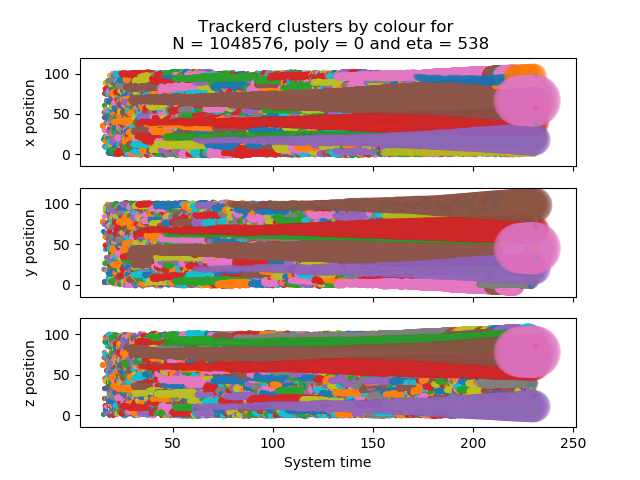
\includegraphics[width=0.6 \linewidth]{cluster_tracking_example.png}
\caption[Individual cluster tracking example]{Example results of cluster tracking algorithm in a monodisperse simulation. The three plots are the projections of the box onto the three spatial dimensions over time. Each cluster is given a color which does not change over time. With it we can see for example that two clusters mingling in one projection are actually some distance apart from each other in an other dimension.\\
While in this example only small metastable clusters that dissolve after some time are present, also nucleation events can be seen in this kind of plot. These are easily identfied as the linewidht of the lines are drawn proportional to the diameter of a sphere with a volume corresponding to the clusters volume under the assumption of a spherical cluster.}
\label{fig:cluster_tracking_example}
\end{figure}

Information about the lifetime and size of the fluctuations derived from the analyzed example trajectory shown in \autoref{fig:cluster_tracking_example} are depicted in \autoref{fig:lifetime}.
\begin{figure}[h]
\centering
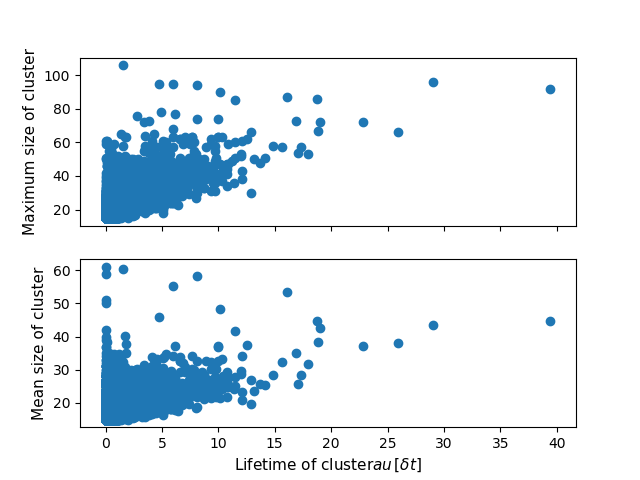
\includegraphics[width=0.6 \linewidth]{cluster_tracking_lifetime.png}
\caption[Example for correlation between a unstable cluster's size and lifetime]{Example of lifetime depending on  maximum (top) or mean (bottom) size of the metastable cluster. }
\label{fig:lifetime}
\end{figure}
First we note that both the maximum size and the mean size can be used as a measure for the scale of the flucutations, as the results do not vary by a lot. Further we can read from the diagram that at a volume fraction of $\eta = 53.4\%$ there are a lot of small to medium sized clusters with short lifetimes up to about $10 \delta t$, and some large clusters with lifetimes of more than $15 \delta t$. The overal impression is that the fluctuation distribution is compact with a small but very far reaching tails towards the large lifetimes as well as towards the large cluster sizes.
